\documentclass[portrait, plainsections]{sciposter}

\usepackage{amsmath}
\usepackage{amssymb}
\usepackage{multicol}
\usepackage{graphicx}
%\usepackage[english]{babel}
\usepackage{alltt}
\usepackage{url}
\usepackage{xspace}
\usepackage{times}
\usepackage{multirow}
\usepackage{algorithm}
\usepackage[noend]{algpseudocode}
% The following doesn't seem to work with multicolumn layouts
%\usepackage{shadethm}
\usepackage{xcolor}
\usepackage{framed}
\usepackage{enumerate}
\usepackage{float}

\usepackage{algorithm}
\usepackage[noend]{algpseudocode}
\usepackage{capt-of}
\makeatletter
\def\BState{\State\hskip-\ALG@thistlm}
\makeatother

\definecolor{BoxCol}{rgb}{0.9,0.9,1}
% uncomment for light blue background to \section boxes 

\definecolor{SectionCol}{rgb}{0,0,0.5}
% uncomment for dark blue \section text 

\setlength{\columnseprule}{0pt}

\colorlet{shadecolor}{orange!15}

\makeatletter
\newcommand{\xRightarrow}[2][]{An example of \ext@arrow 0359\Rightarrowfill@{#1}{#2}}
\makeatother

\renewcommand{\Huge}{\fontsize{55.83}{45}\selectfont}
\renewcommand{\titlesize}{\veryHuge}
\renewcommand{\authorsize}{\Large}

\newcommand{\SR}{\ensuremath{S_{R}}\xspace}
\newcommand{\asrt}{AgentSpeak(RT)\xspace}
\newcommand{\ASRT}{AS(RT)\xspace}%
\newcommand{\pmax}{priority-maximal\xspace}
\newcommand{\etp}{\ensuremath{et}}
\newcommand{\SU}{\emph{SA}$_U$\xspace}
\newcommand{\SAM}{\emph{SA}$_M$\xspace}
\newcommand{\SP}{\ensuremath{S_{P}}\xspace}

\newcommand{\eg}{e.g.,\xspace}
\newcommand{\ie}{i.e.,\xspace}
\newcommand{\etc}{etc\@.\xspace}

\newcommand{\SA}{\emph{SA}\xspace}
\newcommand{\pa}{primitive action\xspace}
\newcommand{\pas}{primitive actions\xspace}

\newtheorem{theorem}{Theorem}
\newtheorem{definition}{Definition}
%\newshadetheorem{theorem}{Theorem}
%\newshadetheorem{definition}{Definition}
%\noleftlogo
%\norightlogo
% \leftlogo[0.8]{logoZJUT.pdf}{logoUoN.png}
% \rightlogo[0.8]{UU_logo2.pdf}{RMIT_University_Logo.png}
\title{Intention Progression with Maintenance Goals}

% These don't seem to affect caption placement.
\setlength{\abovecaptionskip}{0pt}
\setlength{\belowcaptionskip}{0pt}

% The following is a mess, but seems to be the only simple way of getting the authors centred.
\author{\parbox{9.6cm}{\centering Di Wu} \hfill  
\parbox{9.6cm}{\centering Yuan Yao} \hfill 
\parbox{9.6cm}{\centering Natasha Alechina} \hfill 
\parbox{9.6cm}{\centering Brian Logan} \hfill 
\parbox{9.6cm}{\centering John Thangarajah} \hfill}

\institute{\parbox{9.6cm}{\centering Zhejiang University of Technology \\
    \centering wudi@zjut.edu.cn} \hfill  
\parbox{9.6cm}{\centering University of Nottingham Ningbo\\
    \centering n.a.alechina@uu.ul} \hfill 
\parbox{9.6cm}{\centering Utrecht University\\
    \centering n.a.alechina@uu.ul} \hfill 
\parbox{9.6cm}{\centering Utrecht University\\
    \centering b.s.logan@uu.nl} \hfill 
\parbox{9.6cm}{\centering RMIT University \\
    \centering john.thangarajah@rmit.edu.au} \hfill}

% The following commands can be used to alter the default logo settings
%\leftlogo[0.9]{chenille}{  % defines logo to left of title (with scale factor)
%\rightlogo[0.52]{RuGlogo}  % same but on right

\begin{document}


% define conference poster is presented at (appears as footer)
\conference{Proceedings of the Twenty-Ninth International Joint Conference on Artificial Intelligence (IJCAI-20)}

\maketitle

%\begin{figure*}[b]
%\centering
%\includegraphics[width= 1\textwidth]{blocks.pdf}

%\vspace*{4mm}
%\centerline{\textit{Goal-plan tree for the Blocks World domain}}
%\end{figure*}


%%% Begin of Multicols-Environment
\begin{multicols}{3}
In this paper, we propose \SAM, a Monte-Carlo Tree Search (MCTS)-based solver for intention progression problem with both achievement and maintenance goals. We evaluate the performance of our approach in a range of benchmark scenarios with increasing difficulty. The results suggest that \SAM significantly improves the performance of agents with maintenance goals.


\section*{Intention Progreesion For BDI Agent}

\begin{figure}[H]
% \centerline{\includegraphics[width = 1\textwidth]{BDI_model.pdf}}
\end{figure}

\begin{shaded}
\begin{itemize}
\item \textit{Plan selection:} the problem of choosing which plan to the goal 
\item \textit{Intention selection:} the problem of deciding which intention to execute
\item \textit{Inention progression problem(IPP):} Intention selection + Plan selection
\end{itemize}
\end{shaded}

\begin{figure}[H]
% \centerline{\includegraphics[width = 1\textwidth]{example.pdf}}
\end{figure}

\begin{itemize}
\item \textit{goal-plan tree(gpt):} a hierarchical tree structure to represent the relationship between goal, plans and action and all the way to achieve a top-level goal
\item \textit{intention:} The agent's current intentions are represented by a set of pairs, $I = \{(t_1, s_1), \ldots, (t_n, s_n)\}$, where each $t_i \in T$ is a goal-plan tree corresponding to a top-level goal of the agent, and $s_i \in S$ is the \emph{current step} of $t_i$. 
\begin{shaded}
\item \textit{IPP with gpts:} the problem of choosing a current step $s_i \in S$ to progress and decide how to progress it (e.g., if $s_i$ is a (sub)goal, the problem also involves choosing a plan to achieve it) at each deliberation cycle so as to maximise the number of goals achieved (or other utility). 
%If $s_i$ is a (sub)goal, the probem involves choosing a plan for the (sub-)goal and returning the first action step in achieving it. 
\end{shaded}
\end{itemize}


\section*{Maintenance Goals}
% @Extend: Maybe this section can be extended by adding the formal representation of maintenance goals.
Maintenance goals are goals that specify a state of the environment an agent should maintain.
We Consider two ways of implementing maintenance goals: 

\begin{shaded}
\begin{itemize}
\item \textit{Proactive Maintenance Goals:} If the violation of a maintenance goal can be reliably predicted, given the agent's other intentions, the agent can adopt a recovery plan to prevent the maintenance goal from being violated.

\item \textit{Reactive Maintenance Goals:} If the violation of a maintenance goal cannot be reliably predicted, the agent must adopt a recovery plan \textbf{reactively}, i.e., after the violation occurs.
\end{itemize}
\end{shaded}

\begin{figure}[H]
% \centerline{\includegraphics[width = 1\textwidth]{UBexample.pdf}}
\end{figure}

\section*{\SAM Scheduler}

\begin{figure}[H]
% \centerline{\includegraphics[width = 1\textwidth]{mcts-nodeJT.pdf}}
\end{figure}

Each iteration of the \SAM algorithm consists of 4 phases: selection, expansion, simulation and back-propagation.

\begin{figure}[H]
% \centerline{\includegraphics[width = 1\textwidth]{sp-mcts}}
\end{figure}

\vspace*{-4mm}
\centerline{\textit{An iteration of the \SAM algorithm}}
%\vspace{4mm}

As with MCTS and \SA, each iteration of \SAM consists of four main phases: selection, expansion, simulation and back-propagation.

\begin{description}
\item[Selection:] Starting from the root node, we recursively follow child nodes with highest UCT value until a leaf node $n_e$ is reached.

\item [Expansion:] $n_e$ is expanded by creating all its child nodes which correspond to all possible action executions, and adding them to the search tree. 
\item[Simulation:]  One of the newly created child nodes, $n_s$, is selected at random. The value of the state in $n_s$ is estimated by performing $\beta$ pseudorandom simulations.
\item [Back-propagation:] All the simulation value is then \emph{back-propagated} from the simulated states to all states on the path to the initial state. 

To support maintenance goals, we modified the expansion and simulation phases of \SA:
We add additional functionality to deal with maintenance goals.
\begin{shaded}
% \paragraph*{Modification to the Expansion phase:}
% \begin{algorithm}
  % \caption{Modification to the expansion phase}\label{alg:expansion}
  \begin{algorithmic}
    \Function{expand}{$n_e$}
      \State $N \gets \emptyset$
      \State $G_m \gets getMaintenanceGoals()$
      \If{$satisfied(G_m)$ and has no achievement goals}
      \State $continue$

      \EndIf
    \For{each $g \in G_m$}
      \If{one recovery plan for $g$ is already adopted}
        \State $continue$
      \EndIf
      \If{$(isRMG(g)$ and $isViolated(g, n_e))$ or $isPMG(g)$}
        \State $Act \gets getExecutableActions(g)$
          \For{each $a \in Act$}
            \State $n^{\prime} \gets genNode(n_e, a)$
            \State $N \gets N \cup \{n^{\prime}\}$
          \EndFor
      \EndIf
    \EndFor
    \State $n_e.setChildren(N)$
    \For{each $n_i \in N$}
    \State $n_i.setParent(n_e)$
    \EndFor
    
    \EndFunction
  \end{algorithmic}
% \end{algorithm}
\end{shaded}

\begin{shaded}
% \paragraph*{Modification to the Expansion phase:}
% \begin{algorithm}
  % \caption{Modification to the expansion phase}\label{alg:expansion}
  \begin{algorithmic}
    \Function{$simulate$}{$n$}
      \State $N \gets expand(n)$
      \If{$N \neq \emptyset$}
        \State $n \gets random(N)$
        \State $simulate(n)$
      \EndIf
      \Return $n$
    \EndFunction
  \end{algorithmic}
% \end{algorithm}
\end{shaded}

\begin{figure}[H]
% \centerline{\includegraphics[width = 0.5\textwidth]{back.pdf}}
\end{figure}
\end{description}

After $\alpha$ iterations, the step that leads to the best child $n_{b}$ of the root node $n_0$ is returned.

\section*{Evaluation}

We evaluate the performance of \SAM based on a Mars rover example \cite{DuffHT06}. The environment is a grid consisting of 20 $\times$ 20 cells (see Figure \ref{fig:marsrover}).

\begin{center}\vspace{1cm}
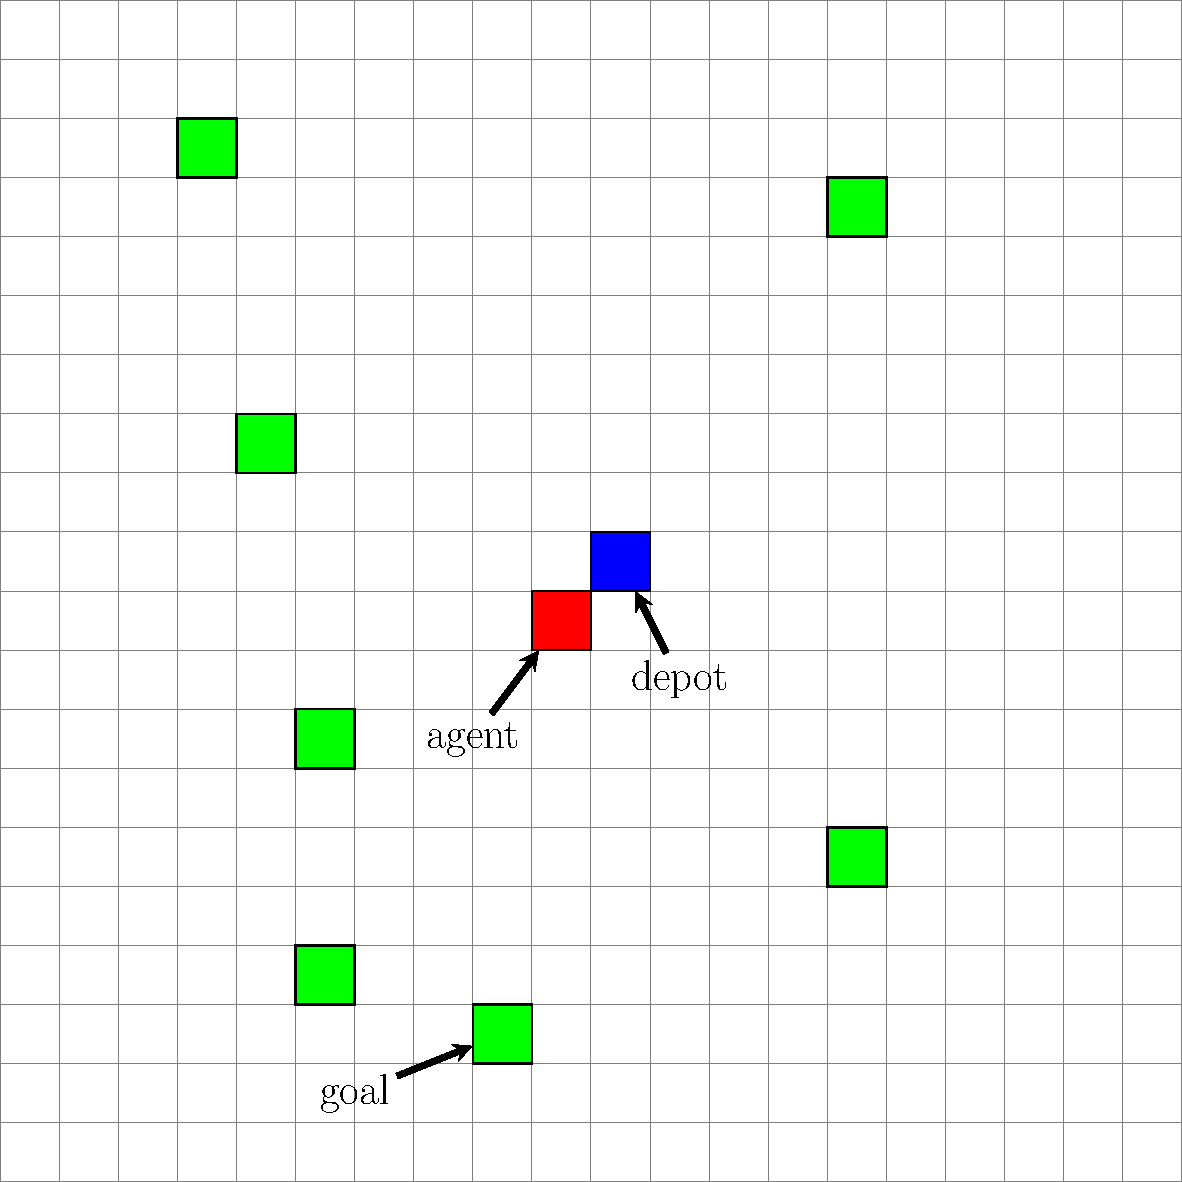
\includegraphics[scale=1]{./figs/mg_example.pdf}
\captionof{figure}{A Mars rover example}
\label{fig:marsrover}
\end{center}\vspace{1cm}
% introduction to the Mars rover example
Each cell in the grid is a location represented as a pair of integer numbers (x, y), where x and y are the x-axis and y-axis values respectively.
%
% We assume the cell at the bottom-left corner is (0, 0) and the one at the top-right corner is (19, 19).
% 
A Mars rover can move up, move down, move left and move right, and is asked to visit different locations in the grid.
There are four actions the Mars rover agent can take to change its current locations, i.e., moveUp, moveDown, moveLeft and moveRight.%, which moves the Mars rover one cell up, down, left, and right respectively. 
% 
%In addition, each movement action will consume 1 unit of battery power. The Mars rover can move to the depot at the center to recharge its battery.
%

In all the experiments reported below, we assume the Mars rover starts in the depot cell, and all its goals (i.e., where to visit) are randomly generated.
% measuring the agent
We measure the performance of the Mars rover agent based on two criteria: the number of goals achieved and the amount of battery consumed.
% That is, the performance of the agent will first be evaluated based on the number of achievement goals achieved (the more the better), if the same number of goals are achieved by different agents, we then compare their battery consumption for achieving the goals (the less the better).
To evaluate the performance of \SAM, the experiments were conducted in 4 cases: RMG, PMG, RMCTS and PMCTS.
%
Both RMG and PMG are from \cite{DuffHT06}.
%
%NMG means no maintenance goals: it assumes movement does not consume battery power. The agent achieves its goals in a FIFO manner.
%
%In the case of RMG, maintenance goals are handled reactively. When this reactive maintenance goal is triggered, the rover must first head to the depot to recharge its battery before attempting to achieve other goals.
%
%On the other hand, maintenance goals are handled proactively in PMG. The maintenance condition is predicted by using summary information. 
%
%NMCTS, as NMG, assumes no maintenance goals, but the goals are scheduled using the \SA scheduler.
%
%Both RMCTS and PMCTS use \SAM to schedule the progression of the agent's intentions. In RMCTS the maintenance goals are implemented reactively and in PMCTS proactively. 


%In the experiments, the \SAM and \SA schedulers are configured to perform 100 iterations in each deliberation cycle and 10 simulations per iteration; we report the average performance in 100 runs. The utility function is set to be $\#goals + \frac{1}{1 + \text{\emph{battery}}}$, where $\#goals$ is the number of goals achieved and \emph{battery} represents the amount of battery used to achieve the goals. We use the amount of battery consumption as additional measure of performance since all the approaches can achieve all goals. We set the battery capacity of the agent to 40 and vary the number of goals to be achieved from 1 to 15.
%
%The reactive maintenance condition is set to be \emph{batteryLevel} $> 20$. 
 %
%For proactive maintenance goals, the condition is set to be \emph{batteryLevel} greater than the minimal number of moves required for the agent to move back to the depot from its current position.

The results are shown in Figure \ref{fig:static1}.

\begin{center}\vspace{1cm}
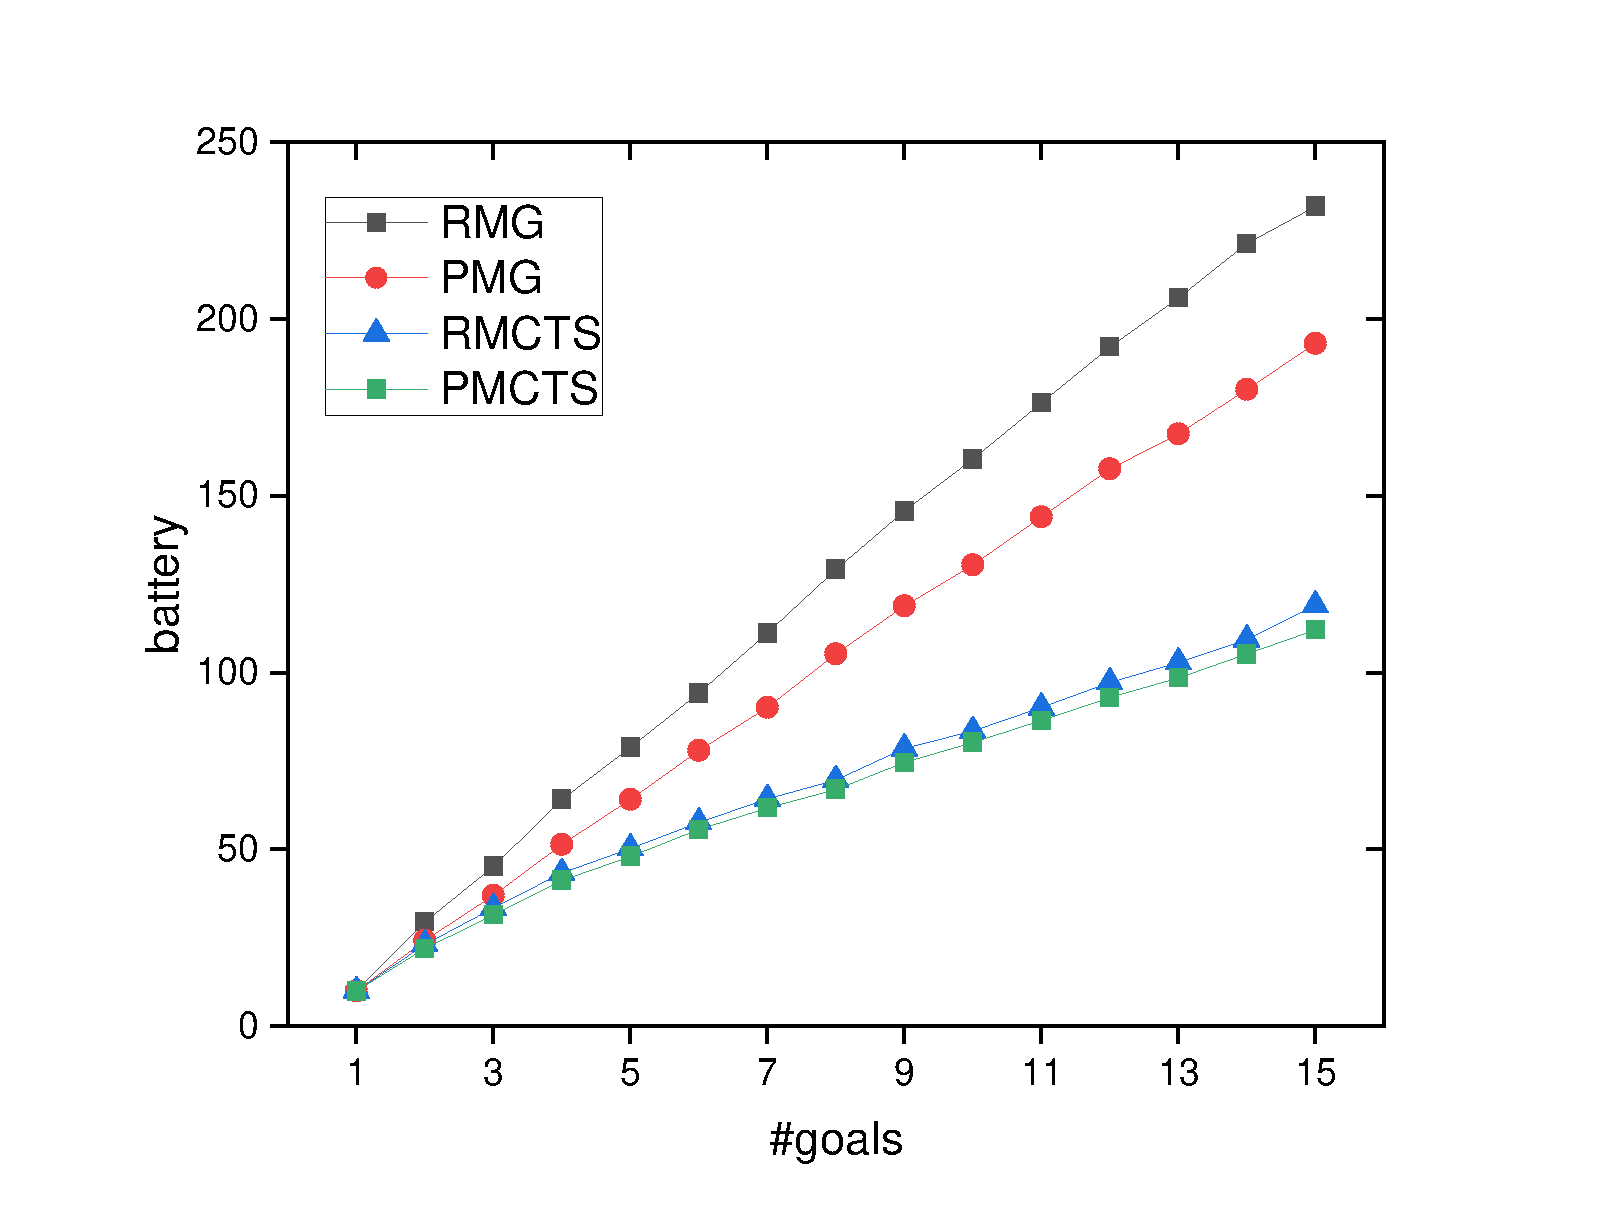
\includegraphics[scale=1]{./figs/gX_cY_fixCap40.pdf}
\captionof{figure}{Battery consumptions with fixed capacity of 40}
\label{fig:static1}
\end{center}\vspace{1cm}

As can be seen, for all approaches the amount of battery consumption increases, as the number of goals increases.
% two baseline
% Natasha: I don't understand the next (commented out) sentence
% general
MCTS-based approaches (PMCTS, and RMCTS) outperform all other approaches, and approaches using proactive maintenance goals have better performance than those using reactive maintenance goals.
%NMCTS has the best performance as it does not consider any battery consumption.
% NMG Natasha: is it NMG or RMG? (comment NMG and text RMG) 
As expected, RMG has the worst performance in all testing cases, i.e., it consumes more battery power than any other approaches.
% reason Natasha: is it NMG or RMG? Change NMG to RMG below
%This is because RMG can only reactively respond to the maintenance goals, causing possible waste of battery when it tries to achieve a goal that is not achievable given the current amount of battery power.
% PMG Natasha: again changed NMG below to RMG
The PMG has better performance than RMG, as it can estimate the battery consumption before pursuing a goal. If the agent will trigger the maintenance goal half way achieving its next achievement goal, then it will choose to recharge first.
% mcts
Finally, both PMCTS and RMCTS have a clear advantage over PMG. Especially, when the given number of goals becomes larger, the differences between MCTS-based approaches and other approaches are more significant. The reason is that the MCTS-based approach can predict not only the possible violation of maintenance conditions during the execution but also possible synergies between different intentions (i.e., the agent can merge the same actions from different intentions to save time and resources).

\section*{Conclusion}
The preliminary results suggested that even without giving any reliable prediction of future violation, \SAM with reactive maintenance goal can still outperform both reactive and proactive approaches proposed in \cite{DuffHT06} in all cases.

The advantage of using \SAM comes from not only the ability to avoid violation between achievement goals and maintenance goals, but also the nature that MCTS can interleave recovery plans and other intentions so as to avoid negative interaction and to exploit synergies 
%as in \cite{Yao/Logan:16a,Yao//:16a} 
if maintenance goals are implemented proactively.

\section*{Future work}
\begin{itemize}
    \item Extend \SAM scheduler to work with nondeterministic actions in uncertain environment.
    \item Extend the current \SAM to additional richer types of goals that are explicitly represented as Linear Temporal Logic formula.
    \item Investigate how to schedule maintenance goals that are only valid for a period of time.
    \item Investigate how to schedule multiple maintenance goals with different priorities or urgency.
\end{itemize}

\small
\begin{thebibliography}{m}

\bibitem{Logan//:17a}
Brian Logan, John Thangarajah, and Neil Yorke{-}Smith.
\newblock {Progressing intention progression: {A} call for a goal-plan tree
  contest.}
\newblock {\em 16th Conference on Autonomous Agents and MultiAgent Systems}, pages 768--772. IFAAMAS, 2017.

\bibitem{yao//:16b}
Y.~Yao and B.~Logan .
\newblock {Action-Level Intention Selection for {BDI} Agents.}
\newblock {\em AAMAS-16}, 1227-1236, 2016.


\end{thebibliography}


\end{multicols}


\end{document}